\section{Experiments}\label{chapter4}

\subsection{Dataset}
We illustrate our two \textsc{nmf} algorithms on two real-world face image datasets: ORL and Extended YaleB (\citet{belhumeur1997eigenfaces}).
Both ORL and Extended YaleB datasets contain multiple images of distinct subjects with various facial expression, lighting condition, and facial details.
Images in ORL are cropped and resized to $92 \times 112$ pixels. We further rescale it to $30 \times 37$ pixels. Similarly, we reduce the size of images in Extended YaleB to $42 \times 48$ pixels.
For each dataset, we flatten the image matrix into a vector and append them together to get a matrix $V$ with shape $d\times n$ where integer~$d$ is the number of pixels in one image and integer~$n$ is the number of images. In each epoch, we use 90\% of data.

\subsection{Noise}
We implement three kinds of noises including Gaussian noise, Poisson noise and Salt \& Pepper noise.
\subsubsection{Gaussian Noise}\label{sec:gau}
We design the Gaussian noise by normal distribution with $0$ mean and $80$ standard deviation (Algorithm~\ref{gau}). The \texttt{ORL} dataset has a global pixel mean of $40$ and the \texttt{CroppedYale} data set has that of $70$. Hence the designed Gaussian noise contaminates the images significantly. We choose the standard deviation to be $80$ so that our Gaussian noise are less likely to coincident with the designed Poisson noise. To satisfy the nonnegative constant, negative value in contaminated image is set to zero.
\begin{lstlisting}[caption= Gaussian Noise Design, label=gau]
def normal(subVhat):
    """Design a Gaussian noise."""
    V_noise = np.random.normal(0, 80, subVhat.shape) #* np.sqrt(subVhat)
    V = subVhat + V_noise
    V[V < 0] = 0
    return V, V_noise
\end{lstlisting}


\subsubsection{Poisson Noise}\label{sec:poi}
The Poisson noise is not additive and has no hyperparameters to be set. Unlike Gaussian noise, contaminated images are drawn directly from Poisson distribution with parameter set to be pixel values. Then, the Poisson noise is calculated from the difference between the contaminated image and the original image, as discussed in Section~\ref{chapter2} and demonstrated in algorithm~\ref{poi}.
\begin{lstlisting}[caption= Poisson Noise Design, label=poi]
def possion(subVhat):
    """Design a Possion noise."""
    V = np.random.poisson(subVhat)
    V_noise = V-subVhat
    return V, V_noise
\end{lstlisting}


\subsubsection{Salt \& Pepper Noise}\label{sec:sal}
% JOYCE please add here
Salt \& Pepper noises are added by drawing random integers from discrete uniform distribution of the interval $[$0, 255$)$ . We find bright place in generated image and replace pixel values in same place of original image with brightest value. Similarly, we also find the dark pixels in generated image and replace pixel values in same place of original image with darkest pixel value. In this case, we set the pixels whose value being greater than or equal to 230 as bright pixels and pixels whose value being less than or equal to 20 as dark pixels.
\begin{lstlisting}[caption= Salt and Pepper Noise Design, label=salt]
def salt_and_pepper(subVhat):
"""Design a salt and pepper noise where make some pixel value zeros."""
  V_noise = np.random.randint(low=0, high=255, size=subVhat.shape, dtype=int)
  V = subVhat.copy()
  V[V_noise <= 20] = 0
  V[V_noise >= 230] = 255
  return V, V_noise
\end{lstlisting}

\subsection{Experiment Setup}

We apply two algorithms (\textsc{nmf} and \textsc{klnmf}) with four categories of noises (no noise, Gaussian noise, Poisson noise and Salt \& Pepper noise), which results in eight combinations in each epoch. In each epoch, we randomly select 90\% of samples to train NMF algorithms and evaluate three metrics on reconstructed images. The training will terminate when the error reaches the minimum error, or the maximum iteration is reached. The minimum error and maximum iteration are hyperparameters which we learn from iterative experiments. Our code saves the learning errors versus number of iterations so that we could draw the plot and observe the convergence of learning process. We increase the number of epochs and calculate the average metrics and confidence intervals.


\subsection{Experiments Results}
Figure~\ref{noisesnmff} and~\ref{noisesklnmff} visualise the original image, designed noises, corrupted images and reconstructed images from left to right. From top to bottom, the four rows correspond to no noise, Gaussian noise discussed in Section~\ref{sec:gau}, Poisson noise discussed in Section~\ref{sec:poi} and Salt \& Paper noise discussed in Section~\ref{sec:sal}.
The first row of Figure~\ref{noisesnmff} and~\ref{noisesklnmff} shows both algorithms reconstructed the original image well without artificial noise and with Poisson noise.
\begin{figure}
	\centering
	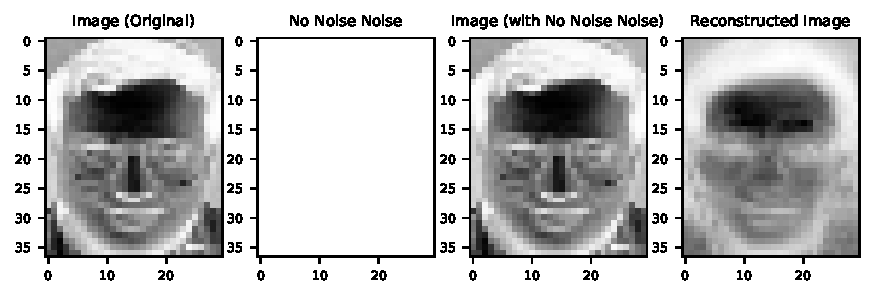
\includegraphics[scale=.9]{Result_Multiplication_Euclidean_No_Noise_Comparison}\\
	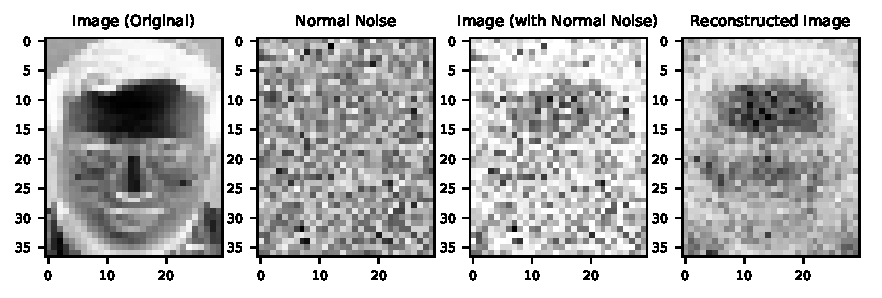
\includegraphics[scale=.9]{Result_Multiplication_Euclidean_Normal_Comparison}\\
	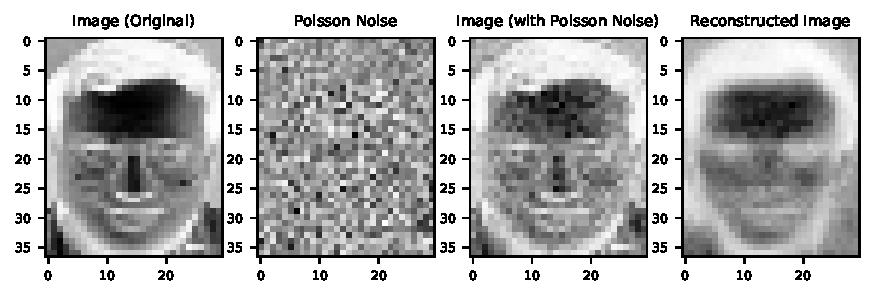
\includegraphics[scale=.9]{Result_Multiplication_Euclidean_Poisson_Comparison}\\
	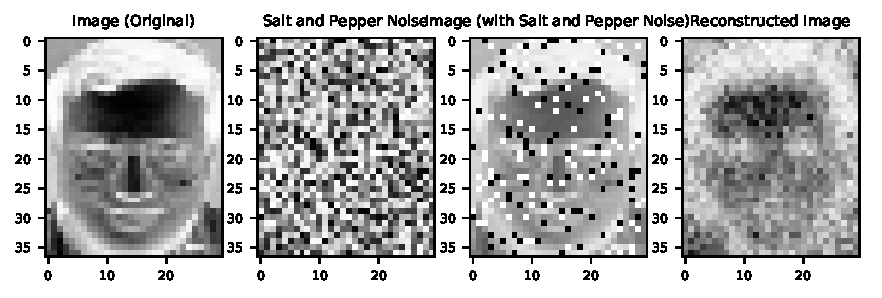
\includegraphics[scale=.9]{Result_Multiplication_Euclidean_Salt_and_Pepper_Comparison}
	\caption{The reconstructed image by \textbf{nmf}. The original images (Column~1) are combined with noises (Column~1) including Gaussian Noise with Variance~$80$ (Row~2), Poisson Noise (Row~3), and Salt \& Pepper Noise (Row~4). The corrupted images are shown in Column~3. The reconstructed images are shown in (Column~4). The reconstruction with no noise is shown in Row~1.}\label{noisesnmff}
\end{figure}
\begin{figure}
	\centering
	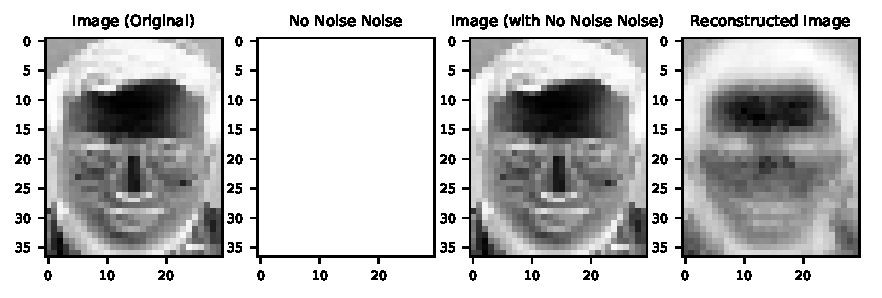
\includegraphics[scale=.9]{Result_Multiplication_KL_Divergence_No_Noise_Comparison}\\
	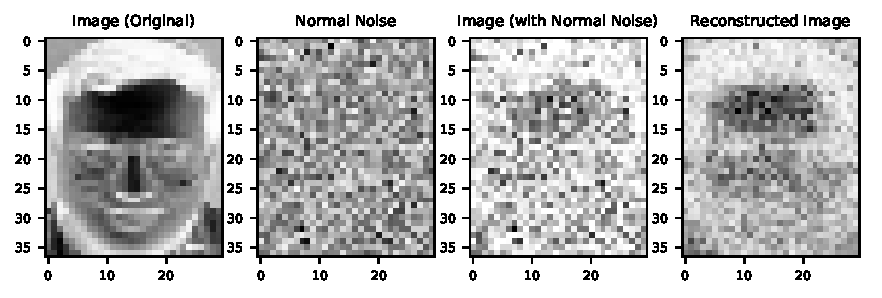
\includegraphics[scale=.9]{Result_Multiplication_KL_Divergence_Normal_Comparison}\\
	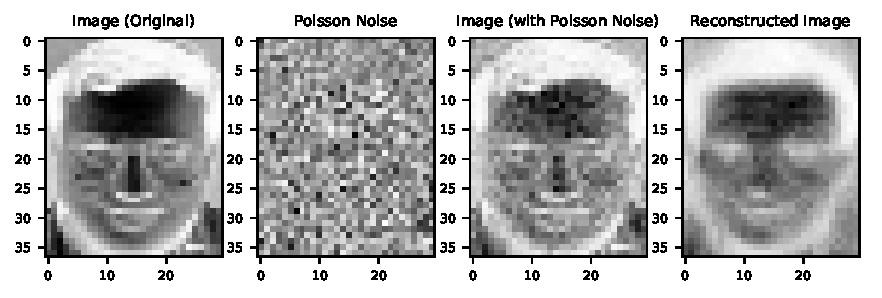
\includegraphics[scale=.9]{Result_Multiplication_KL_Divergence_Poisson_Comparison}\\
	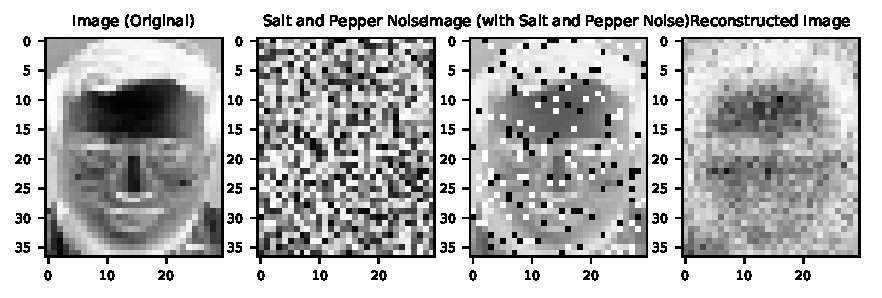
\includegraphics[scale=.9]{Result_Multiplication_KL_Divergence_Salt_and_Pepper_Comparison}
\caption{The reconstructed image by \textbf{klnmf}. The original images (Column~1) are combined with noises (Column~1) including Gaussian Noise with Variance~$80$ (Row~2), Poisson Noise (Row~3), and Salt \& Pepper Noise (Row~4). The corrupted images are shown in Column~3. The reconstructed images are shown in (Column~4). The reconstruction with no noise is shown in Row~1.}\label{noisesklnmff}
\end{figure}
However, when the noise is large (the second and last rows in Figure~\ref{noisesnmff} and~\ref{noisesklnmff}), the quality of reconstructed images are only marginally better than the contaminated images.
Our result is consistent with \citet{guan2017truncated}, who assert that \textsc{nmf} may fail to handle extremely corrupted images when assumed distribution of noise is violated.
Moreover, the difference between images generated by \textsc{nmf} and \textsc{klnmf} are not visually significant.
Hence, we implement statistical hypothesis test to compare of \textsc{rre}s of the two algorithms.

Substitute \href{https://raw.githubusercontent.com/JoyceXinyueWang/nmf_raw_data/master/raw_result_acc.csv}{\textsc{rre} results} from $80$ simulations of the two algorithms into Kolmogorov-Smirnovs test~\eqref{teststatistic} gives test statistics~$D=1, 1 ,0.6625$ with no noise, Gaussian noise, and Poisson noise, for the \textsc{orl} dataset. These three test statistics are all much greater than the critical value~$0.215$. Hence there are strong evidence that the performance of \textsc{nmf} and \textsc{klnmf} are different in these three problems. For salt and Pepper noise, test statistic~$D=0.2125<0.215$, hence we fail to conclude that the two methods have different robustness against Salt and Pepper noise. Further one tail Kolmogorov-Smirnov test concludes that \textsc{klnmf} performs better reconstructing the original image with no noise and is more robust Poisson noise.
In contrast, \textsc{nmf} is more robust against Gaussian noise, even with only $500$ iterations ($1200$ for \textsc{klnmf}). Hence, \textsc{nmf} is clearly more robust than \textsc{klnmf} against Gaussian noise.

Theoretical results discussed in Section~\ref{chapter2} suggest \textsc{nmf} is more robust against Gaussian noise whereas \textsc{klnmf} is more robust against Poisson noise. Our experimental results concluded from Kolmogorov-Smirnovs hypothesis tests agree with these theoretical results. Further, as both of the algorithms are not designed for Salt and Pepper noise, they have similar performance against it.

These results can be observed by directly reading whether the confidence intervals overlap in table~\ref{tab:ci}. Also, the statistical results agree with the visualisation in Figure~\ref{noisesnmff} and~\ref{noisesklnmff}. These results can be intuitively understood---also the differences in the robustness of the two algorithms are small, the even smaller variances in the \textsc{rre} results make them statistically different under Poisson and Gaussian noise.

In terms of the cropped Yale dataset, results from hypothesis tests show that \textsc{nmf} performs uniformly better than \textsc{klnmf}, suggesting more iterations are required on \textsc{klnmf} to compare these two algorithms fairly. We fail to do so because the dataset is much larger than \textsc{orl} and our multiplicative update rules, especially for \textsc{klnmf} converge too slow.

\begin{table}
\caption{Average of evaluations metrics over 80 simulations using the \textsc{orl} dataset. The 95\% confidence intervals are calculated using bootstrap.}
\hspace{-1cm}{\small
\label{tab:ci}\begin{tabular}{l|lll}
 \hline
\textsc{orl} dataset & \textsc{rre} & \textsc{acc} & \textsc{nmi}\tabularnewline
 \hline
\textsc{nmf} no noise & 0.1583 (0.1581, 0.1584) & 0.7364 (0.731, 0.742) & 0.8536 (0.8506, 0.8567)\tabularnewline

\textsc{nmf} Gaussian noise & 0.2925 (0.2922, 0.2927) & 0.447 (0.4423, 0.4521) & 0.6212 (0.6176, 0.6247)\tabularnewline

\textsc{nmf} Poisson noise & 0.1611 (0.161, 0.1613) & 0.7313 (0.7262, 0.7367) & 0.8493 (0.8456, 0.8527)\tabularnewline

\textsc{nmf} Salt and Pepper noise & 0.2636 (0.2634, 0.2638) & 0.5094 (0.504, 0.5151) & 0.6721 (0.6679, 0.6764)\tabularnewline

\textsc{klnmf} no noise & 0.1729 (0.1728, 0.173) & 0.7406 (0.7352, 0.7458) & 0.8599 (0.8568, 0.8632)\tabularnewline

\textsc{klnmf} Gaussian noise & 0.2977 (0.2976, 0.2979) & 0.4538 (0.4483, 0.4595) & 0.6209 (0.6165, 0.6255)\tabularnewline

\textsc{klnmf} Poisson noise & 0.1602 (0.1601, 0.1603) & 0.7417 (0.7365, 0.7472) & 0.8573 (0.8542, 0.8602)\tabularnewline

\textsc{klnmf} Salt and Pepper noise & 0.264 (0.2638, 0.2643) & 0.5089 (0.5038, 0.5139) & 0.6734 (0.6694, 0.6779)\tabularnewline
 \hline
\end{tabular}}
\end{table}

\subsubsection{{CroppedYale} Evaluations metrics FAKE FOR NOW}
\begin{table}
\caption{Average of evaluations metrics over 40 simulations using CroppedYale data set. The 95\% confidence intervals are calculated using bootstrap.}
\hspace{-1cm}{\small
\begin{tabular}{l|lll}
 \hline
\textsc{orl} dataset & \textsc{rre} & \textsc{acc} & \textsc{nmi}\tabularnewline
 \hline
\textsc{nmf} no noise & 0.1583 (0.1581, 0.1584) & 0.7364 (0.731, 0.742) & 0.8536 (0.8506, 0.8567)\tabularnewline

\textsc{nmf} Gaussian noise & 0.2925 (0.2922, 0.2927) & 0.447 (0.4423, 0.4521) & 0.6212 (0.6176, 0.6247)\tabularnewline

\textsc{nmf} Poisson noise & 0.1611 (0.161, 0.1613) & 0.7313 (0.7262, 0.7367) & 0.8493 (0.8456, 0.8527)\tabularnewline

\textsc{nmf} Salt and Pepper noise & 0.2636 (0.2634, 0.2638) & 0.5094 (0.504, 0.5151) & 0.6721 (0.6679, 0.6764)\tabularnewline

\textsc{klnmf} no noise & 0.1729 (0.1728, 0.173) & 0.7406 (0.7352, 0.7458) & 0.8599 (0.8568, 0.8632)\tabularnewline

\textsc{klnmf} Gaussian noise & 0.2977 (0.2976, 0.2979) & 0.4538 (0.4483, 0.4595) & 0.6209 (0.6165, 0.6255)\tabularnewline

\textsc{klnmf} Poisson noise & 0.1602 (0.1601, 0.1603) & 0.7417 (0.7365, 0.7472) & 0.8573 (0.8542, 0.8602)\tabularnewline

\textsc{klnmf} Salt and Pepper noise & 0.264 (0.2638, 0.2643) & 0.5089 (0.5038, 0.5139) & 0.6734 (0.6694, 0.6779)\tabularnewline
 \hline
\end{tabular}}
\end{table}
\subsection{Personal Reflection}
The implementation of this project was challenging and rewarding. We overcome many problems that are not taught in class by research. For instance, we learnt to use parallel computing when the performance of~\textsc{klnmf} was always struggling due to local optimal. 
Moreover, we critically considered what truly defines a `good' algorithm. Although theoretically privileged algorithms may be good for handling difficult tasks, they tend to be time consuming and not easy to implement. For example, through literature review, we found some algorithms such as Truncated Cauchy \textsc{nmf} \citet{guan2017truncated} that are excellent for contaminated data but too difficult for us to implement. We also suffered time-performance tradeoff especially when training Extended YaleB dataset. Hence, in real-world practice, simpler and faster algorithm may be more widely used than advanced algorithms. 
Lastly, we observed many interesting results during the experiment. For instance, we found that the \textsc{rre}s of \textsc{nmf} and \textsc{klnmf} with Poisson noise is superior than that with no noise. One hypothesis is that added Poisson noise neutralized the noise from original image. Another hypothesis is that this may result from the noise assumptions made by these two algorithms. 
